% Source: graduate-coursework/Prior_Semesters/Fa25/EMCH501/HW3/HW3.tex
% Description: 3D view of the rod with a differential slice between $x$ and $x + \Delta x$.

\documentclass[border=4pt]{standalone}
\usepackage{amsmath}
\usepackage{amssymb}
\usepackage{graphicx}
\usepackage{pgfplots}
\usepackage{tikz}
\usepackage{xcolor}
\pgfplotsset{compat=1.18}
\usetikzlibrary{shapes.geometric, arrows.meta, positioning, decorations.pathmorphing, patterns}

\definecolor{USC_Garnet}{HTML}{73000A}
\definecolor{USC_Sandstorm}{HTML}{FFF2E3}
\definecolor{USC_Black90}{HTML}{565656}
\definecolor{USC_Black10}{HTML}{ECECEC}
\definecolor{USC_Honeycomb}{HTML}{65780B}

\begin{document}
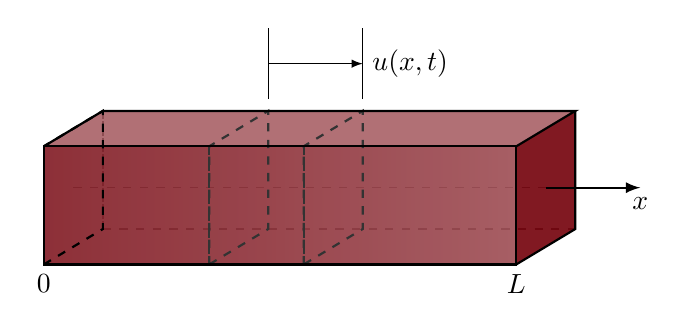
\begin{tikzpicture}[
    x={(1cm,0cm)},       % X direction
    y={(0cm,1cm)},       % Y direction
    z={(0.5cm,0.3cm)},   % Z direction (depth)
    scale=1.5,
    >=Stealth
]

    % --- Parameters ---
    \def\L{4}    % Length of the rod
    \def\H{1}    % Height
    \def\D{1}    % Depth
    \def\sStart{1.4} % Start of slice x
    \def\sEnd{2.2}   % End of slice x+dx

    % --- 1. Hidden (Back) Lines ---
    % Bottom-Back edge and Left-Back vertical edge are hidden
    \draw[dashed, thick, black!70] (0,0,\D) -- (\L,0,\D);
    \draw[dashed, thick, black!70] (0,0,\D) -- (0,\H,\D);
    \draw[dashed, thick, black!70] (0,\H,\D) -- (0,0,\D); % Left back vertical
    
    % --- 2. Centerline Axes (Longitudinal) ---
    % Central axis through the volume
    \draw[dashed, thin, black!60] (0, \H/2, \D/2) -- (\L, \H/2, \D/2);

    % --- 3. The Rod Body (Fills) ---
    
    % We apply shading. Since TikZ standard shading is 2D, we shade faces individually.
    
    % Front Face (Gradient Left to Right)
    \shade[left color=USC_Garnet!90, right color=USC_Garnet!70, opacity=0.9] 
        (0,0,0) rectangle (\L,\H,0);
        
    % Top Face (Lighter uniform yellow)
    \fill[USC_Garnet!70, opacity=0.8] 
        (0,\H,0) -- (\L,\H,0) -- (\L,\H,\D) -- (0,\H,\D) -- cycle;
        
    % Side/Right Face (Darker)
    \fill[USC_Garnet, opacity=0.9] 
        (\L,0,0) -- (\L,\H,0) -- (\L,\H,\D) -- (\L,0,\D) -- cycle;

    % --- 4. The "Slice" / Element Lines ---
    % These are the dashed cuts at x and x+dx
    
    % Slice Start
    \draw[dashed, thick, black!80] (\sStart, 0, 0) -- (\sStart, \H, 0) -- (\sStart, \H, \D) -- (\sStart, 0, \D) -- cycle;
    \draw[dashed, thick, black!80] (\sStart, \H, 0) -- (\sStart, 0, 0); % Front face vertical
    
    % Slice End
    \draw[dashed, thick, black!80] (\sEnd, 0, 0) -- (\sEnd, \H, 0) -- (\sEnd, \H, \D) -- (\sEnd, 0, \D) -- cycle;
    \draw[dashed, thick, black!80] (\sEnd, \H, 0) -- (\sEnd, 0, 0); % Front face vertical

    % --- 5. Visible Edges (Outlines) ---
    \draw[thick] (0,0,0) -- (\L,0,0) -- (\L,\H,0) -- (0,\H,0) -- cycle; % Front face border
    \draw[thick] (0,\H,0) -- (0,\H,\D) -- (\L,\H,\D) -- (\L,\H,0);     % Top edges
    \draw[thick] (\L,0,0) -- (\L,0,\D) -- (\L,\H,\D);                   % Right edges
    \draw[thick, dashed] (0,0,0) -- (0,0,\D) -- (0,\H,\D) -- (0,\H,0);  % Left edges (partially dashed in standard view, but strict outline here)

    % --- 6. Annotations ---

    % Coordinates Labels
    \node[below] at (0,0,0) {$0$};
    \node[below] at (\L,0,0) {$L$};

    % X-Axis Arrow
    \draw[-latex, thick] (\L, \H/2, \D/2) -- ++(0.8, 0, 0) node[below] {$x$};

    % Dimension lines for u(x,t)
    % Extension lines going up
    \draw[thin, black] (\sStart, \H+0.1, \D) -- ++(0, 0.6, 0);
    \draw[thin, black] (\sEnd, \H+0.1, \D) -- ++(0, 0.6, 0);

    % Arrow and Label
    \draw[-latex, thin] (\sStart, \H+0.4, \D) -- node[right, xshift=6mm] {$u(x,t)$} ++(0.8, 0, 0);
    
    % Note: In the original image, the arrow starts at the left slice boundary 
    % and points right, indicating displacement direction.

\end{tikzpicture}
\end{document}
